% INHALT: {{{

% Aufgabenstellung ...
% Begründung des Themas ...
% und Ziele formulieren

% Das Thema wird abgegrenzt,
% die relevanten Arbeiten anderer Autoren werden zitiert,
% und eventuell werden fachliche Grundlagen, welche für das Verständnis des Berichtes nötig sind, erläutert.
% In diesem ersten Abschnitt soll demnach klargemacht werden, worauf der Autor/die Au- torin hinaus will.

%}}}

\subsection{Begründung des Themas} %{{{

Viele Computervision-Anwendungen, welche Einzel- und Mehrkamerasysteme verwenden, sind auf ein korrektes Timing der aufgenommenen Bilder angewiesen.
Dabei gehen die Bilder von der Kamerahardware über den Übertragungsweg zum Auswertesystem (USB (Universal Serial Bus), Ethernet, WiFi, ...) und durch verschiedene Treiberschichten bis in die Anwendung einen langen Weg.
Zwar bieten die Hersteller manchmal einen Zeitstempel für jedes aufgenommene Bild.
Trotzdem wäre ein automatisches Messgerät praktisch, mit dem das Zeitverhalten der Aufnahmen (z.B. Bilder pro Sekunde, Jitter) oder die Synchronität von Mehrkamerasystemen bestimmt werden können.

% END: Begründung des Themas }}}

\subsection{Aufgabenstellung} %{{{

Das Messsystem wird als Elektronik ausgelegt, welche mehrere LEDs (Leuchtdioden) zur Anzeige hat.
Die Kamera schaut auf die LEDs und nimmt diese auf.
Das Messsystem verändert die LEDs zeitabhängig und kodiert einen Zeitstempel in die Zustände der LEDs.
Mittels einer Software sollte man anhand der von der Kamera aufgenommenen Bilder die Zeitstempel rekonstruieren können und mit diesen das Zeitverhalten der Kamera analysieren können.

Das Messsystem sollte sich per USB mit einem PC (Personal Computer) verbinden lassen und von diesem per serielle Schnittstelle konfigurieren lassen (z.B. Messfrequenz).
Es wäre auch gut, wenn das Messsystem einen Triggerausgang und Triggereingang hätte mit dem sich Kameras oder das Messsystem selbst triggern lassen.

% END: Aufgabenstellung }}}


\subsection{Ziele} %{{{

\begin{longtable}[l]{ @{} >{\RaggedRight\hspace{0pt}} lp{.96\linewidth} @{} }
    \textbullet & Mit welcher Anordnung, bzw. Ansteuerung der LEDs kann geschickt Zeit kodiert und detektiert werden?
    \\\textbullet & Welche Kamerafehler und Aufnahmeeigenschaften können detektiert werden?
    \\\textbullet & Wie grob weichen die vom Hersteller versprochenen Aufnahmeeigenschaften ab?
    \\\textbullet & Welche Einflüsse hat eine variierende Bildqualität?
    \addtocounter{table}{-1}
\end{longtable}

%}}}

\subsection{Systemabgrenzung} %{{{

Als erstes wurde eine Systemabgrenzung erstellt, welche in \imgref{img:Systemabgrenzung} zu sehen ist.

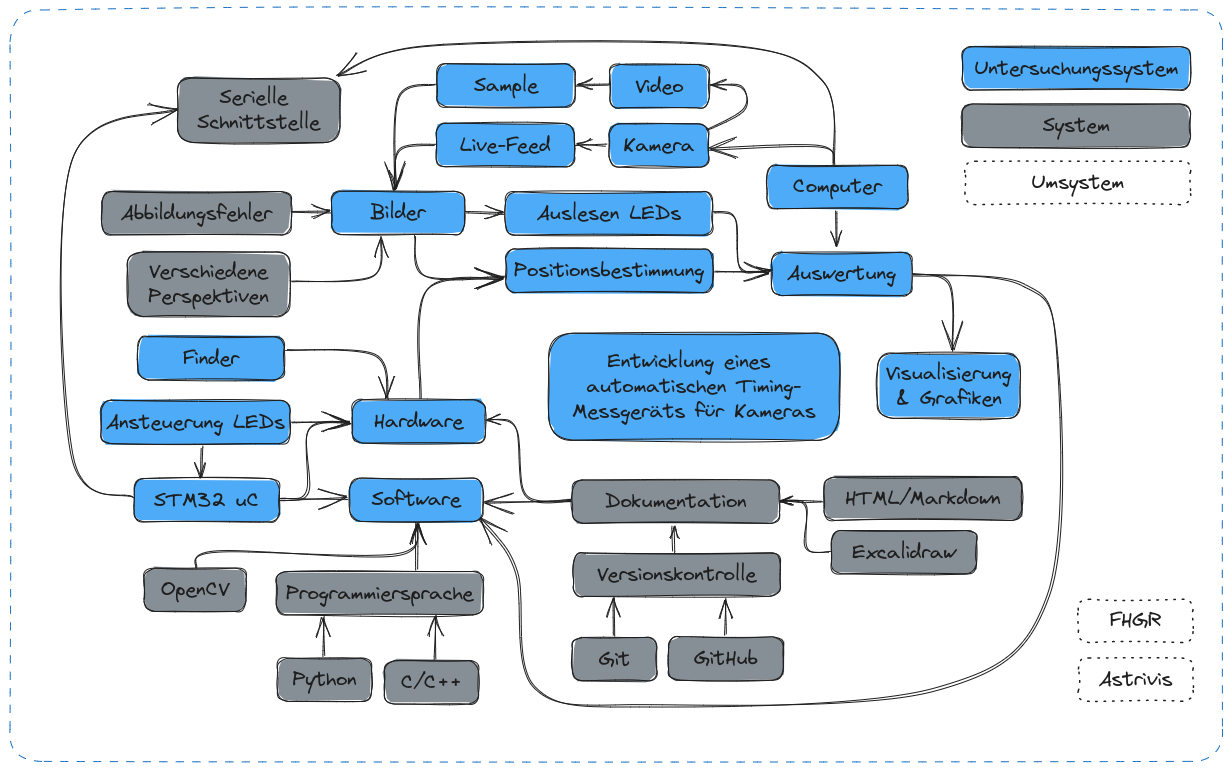
\includegraphics[width=\linewidth]{../images/systemabgrenzung.png}
\vspace{-2.5em}
\captionof{figure}{Systemabgrenzung}
\label{img:Systemabgrenzung}

% END: Systemabgrenzung }}}

\subsection{Relevante Arbeiten} %{{{

Zeitstempel können als Gray-Codes codiert werden.
%
Zur Decodierung und Analyse einer Kamera wird jedoch eine zusätzliche externe Kamera verwendet, die das System von Aussen beobachtet \cite{7836493}.

Die Position, inspiriert durch Data Matrizen \cite{data-matrix}, wird anhand der Anordnung der LEDs bestimmt.

% END: Relevante Arbeiten }}}

\subsection{Fachliche Grundlagen} %{{{

\subsubsection{Pulsweitenmodulation} %{{{

Die Helligkeit einer LED kann durch Variation der Eingangsleistung verändert werden.
%
Oft kann eine LED jedoch nur ein- oder ausgeschalten werden, welches eine Änderung der Helligkeit durch ändern der Stromstärke schwierig gestaltet.
%
Die Eingangsleistung wird demnach über die Zeit durch PWM (Pulsweitenmodulation) des digitalen Ansteuerungssignales kontrolliert reguliert.


Ein Beispiel:
%
Wenn eine LED wiederholend innert kurzer Zeit 25\% an und den Rest der Zeit aus ist, sieht es für einen Betrachter so aus, als leuchte die LED mit einem viertel der vollen Intensität.
%
Dies nennt sich auch 25\% Duty Cycle.

%}}}

\subsubsection{Timer im Mikrokontroller} %{{{

Die Aufgabe eines Timers in einem Mikrokontroller ist das Zählen auf eine bestimmte Zahl.
%
Vorgegeben ist auch die Eingangsgeschwindigkeit und ein Prescaler, welcher die Eingangsgeschwindigkeit dividiert und so die Zählergeschwindigkeit vorgibt.
%
Durch zurücksetzen des Zählers beim Erreichen des Zielwertes wird fortlaufend gezählt.


Der Zeitpunkt beim Erreichen der vorgegebenen Zahl kann somit als variable Frequenzgeneration eingesetzt werden.
%
In \eqref{eq:f_Timer} sind $z_\text{ARR}, z_\text{PSC} \in \mathbb{N}$ die Werte vom Auto-Reload- \& Prescaler-Register.
%
Die Eingangsfrequenz ist durch $f_\text{Eingang}$ gegeben und die resultierende variable Ausgangsfrequenz ist $f_\text{Timer}$.

\begin{equation}\label{eq:f_Timer}
    f_\text{Timer} = \frac{ f_\text{Eingang} }{ \left( z_\text{ARR} + 1 \right) \cdot \left( z_\text{PSC} + 1 \right) }
\end{equation}


\subsubsection{Rolling und Global Shutter}

Das Auslesen der Pixel einer Kamera wird unterschieden zwischen Rolling und Global Shutter.
Beim Global Shutter werden alle Pixelwerte gleichzeitig ausgelesen.
Anders ist dies beim Rolling Shutter, wo zeilenweise Pixelwerte ausgelesen werden \cite{rolling-global}.
%Wobei dies Zeilenweise geschieht beim Rolling Shutter \cite{rolling-global}.


%}}}

% TODO: schieberegister vlt noch hinzufügen?

% END: Fachliche Grundlagen }}}


